\chapter{NumPy}
\label{chp:Numpy}
\epigraph{
	The only thing that remains unsolved is the resolution of the problem.
}{Thomas Wells}

NumPy ist ein Python-Modul mit vielen Einsatzgebieten. Die Dokumentation des Pakets\footnote{\url{https://numpy.org/doc/stable/user/whatisnumpy.html}} wird selbstbewusst eingeleitet mit:
\begin{center}
	\emph{NumPy is the fundamental package for scientific computing in Python.}
\end{center}

Nicht nur werden Routinen für viele häufig auftauchende Aufgaben bereitgestellt; die Umsetzung dieser ist auch bedeutend schneller, als es in \enquote{Vanilla-Python} möglich wäre, da die Kernroutinen in kompilierten C-Libraries vorliegt. Wir erhalten also nicht nur zusätzlichen Komfort, sondern auch einen massiven Speedup bei der Verwendung von NumPy-Funktionen.

\begin{hintbox}[Installation]
Nicht auf allen Systemen ist NumPy sofort vorinstalliert. Um zu testen, ob Ihr System bereits die NumPy-Bibliothek unterstützt, können Sie diesen Code auführen:
\begin{codebox}[Installation von NumPy testen]
\begin{minted}[linenos]{python3}
try:
    import numpy
except ImportError:
    print("numpy is not installed")
else :
    print("numpy is ready for use")
\end{minted}
\end{codebox}

Sollte die Zeile \texttt{numpy is not installed} erscheinen, so können Sie dies einfach nachinstallieren. Rufen Sie hierzu entweder die Anaconda-Konsole auf (Windows, Mac) oder ein reguläres Terminal (Linux). Hier geben Sie die folgende Zeile (Windows, Mac) ein:

\begin{cmdbox}[NumPy Nachinstallieren -- Windows{,} Mac]
\begin{minted}{text}
pip install numpy
\end{minted}
\end{cmdbox}

oder, wenn Sie unter Linux arbeiten:
\begin{cmdbox}[NumPy Nachinstallieren -- Linux]
\begin{minted}{text}
pip3 install numpy
\end{minted}
\end{cmdbox}
\end{hintbox}

Hier kann nur auf die wichtigsten Features eingegangen werden; eine vollständige Referenz finden Sie unter \url{https://numpy.org/doc/stable/numpy-ref.pdf} (1812 Seiten, Stand Juni 2020).

\section{Grundlegendes Objekt}
Für die Arbeit mit NumPy muss natürlich zuerst das Modul geladen werden. Per Konvention geschieht dies mit dem Alias \texttt{np}:
\begin{codebox}[Modul NumPy Laden]
\begin{minted}{python3}
import numpy as np
\end{minted}
\end{codebox}

Zentrales Objekt in allen NumPy-Anwendungen ist das \emph{Numpy-Array}. In erster Näherung verhält es sich wie eine Ihnen bereits bekannte \inPy{list}: NumPy-Arrays sind Container von geordneten Werten, \ie ein Wert im Container kann durch seinen \emph{Index} eindeutig identifiziert werden. Sie können sowohl eindimensionale als auch mehrdimensionale Objekte darstellen, also beispielsweise Tabellen abbilden. Über NumPy-Arrays kann auch iteriert werden, \ie es ist möglich sie mit einer \inPy{for}-Schleife zu durchlaufen.

Im Gegensatz zu Python-\inPy{list}s müssen aber \emph{alle Einträge} in einem Numpy-Array \emph{denselben Datentyp} haben\footnote{Diese Einschränkung macht die zugründeliegende Speicherstruktur sehr viel einheitlicher und ist mit für den großen Geschwindigkeits-Gewinn verantwortlich, den wir mit NumPy erhalten. In der Praxis schränkt uns dies kaum ein, da wir NumPy ohnehin nur für ähnliche Daten verwenden.}. Bei Tabellen und Tensoren müssen alle Einträge angegeben werden; es ist also nicht möglich, eine Tabelle mit 5 Zeilen in der ersten Spalte und 10 Zeilen in der zweiten Spalte anzulegen.

Erzeugt werden NumPy-Arrays über ihren Konstruktor aus normalen Python-\inPy{list}s\footnote{Genauer: Aus einem \emph{Iterable}. Das bedeutet, dass auch \inPy{tuple}s, ... benutzt werden können, um NumPy-Arrays zu erzeugen.}. Wo versucht wird, die Einschränkungen auf gleichen Datentyp oder ausgefüllte Tabellen zu missachten, wendet NumPy verschiedene Strategien an, um ein kompatibles Objekt zu erzeugen:

\begin{codebox}[Beispiel: NumPy-Arrays erzeugen]
\begin{minted}[linenos]{python3}
import numpy as np

npList   = np.array([1, 2, 3])
npMixed1 = np.array([1, 1.5])
npMixed2 = np.array([1, 1.0, "1.0"])

npTab      = np.array([[1, 2, 3], [4, 5, 6]])
npListList = np.array([[1], [2, 3]])

print(npList)
print(npMixed1)
print(npMixed2)
print(npTab)
print(npListList)
\end{minted}
\end{codebox}

\begin{cmdbox}[Ausgabe: NumPy-Arrays erzeugen]
\begin{minted}{text}
[1 2 3]
[1.  1.5]
['1' '1.0' '1.0']
[[1 2 3]
 [4 5 6]]
[list([1]) list([2, 3])]
\end{minted}
\end{cmdbox}

Wir sehen zunächst, dass die aus \inPy{int}s bestehende \inPy{list [1, 2, 3]} direkt als NumPy-Array übernommen werden kann (erste Zeile der Ausgabe). Für die aus einem \inPy{int} und einem \inPy{float} bestehende \inPy{list [1, 1.5]} rechnet NumPy beide Einträge zu \inPy{float}s um\footnote{Genauer zu \texttt{np.float64}s -- siehe etwas später dazu.}. Die \inPy{list [1, 1.0, "1.0"]} enthält einen String; da nicht jeder String in eine Zahl umgewandelt werden kann, haben die Entwickler von NumPy sich dazu entschieden, dass in so einem Fall \emph{alle Einträge} zu Strings umgewandelt werden.

Im Falle von Tabellen wie der \inPy{list [[1, 2], [3, 4]]} werden die verschachtelten Listen in das interne Schema der NumPy-Bibliothek heruntergebrochen. In diesem Format kann die Tabelle auch \enquote{schön} als Tabelle ausgegeben werden -- ein einziger \inPy{print}-Befehl erzeugt mehrere Zeilen auf dem Bildschirm.

Dagegen ist \inPy{list [[1], [2, 3]]} keine vollständig ausgefüllte Tabelle; NumPy fasst sie daher als Array von \inPy{list}s auf. Die Ausgabe spiegelt genau dies wieder.

\subsection{Datentypen und Attribute des NumPy-Arrays}
Der Speicherbedarf für eine Zahl wird in Python dynamisch angepasst. Für kleine Zahlen werden nur einige wenige Bytes verwendet, größere Zahlen beanspruchen einen langen zusammenhängenden Speicherbereich. Hinzu kommt ein \emph{Descriptor}, also ein Speicherabschnitt, in dem deklariert wird, wie viel Speicherplatz zur Darstellung der Zahl verwendet wird, und wo dieser zu finden ist. Der \inPy{int 4} beansprucht \eg 28 Bytes; für den \inPy{int 2**20} dagegen sind es 32 Bytes und für die Zahl \inPy{2**128} werden 44 Bytes belegt. Diese Flexibilität kommt zum Preis längerer Laufzeiten.

In NumPy hingegen wird für alle Zahlen derselbe Speicherplatz zur Verfügung gestellt, der sich aus dem Datentypen herleitet. Für einen \texttt{np.int64} -- die häufigste Übersetzung für einen Python-\inPy{int} -- werden \emph{immer} 8 Bytes genutzt. Es ist offensichtlich, dass 8 Bytes schneller zu verarbeiten sind als 28. Dafür aber kann es beim Rechnen mit NumPy zu sogenannten \emph{oveverflows} kommen: Das Ergebnis einer Berechnung kann zu groß sein, um im bereitgestellten Speicherbereich abgelegt werden zu können. Tabelle \ref{tab:NumPyDataTypes} enthält eine Übersicht der wichtigsten bereitgestellten Typen. Wie Sie an den aufgelisteten Wertebereichen sehen können, sind die Beschränkungen der Wertebereiche selten von Belang.

Unter \url{https://numpy.org/doc/stable/reference/arrays.dtypes.html} finden Sie weitere Details zum Umgang mit den Numpy-Datentypen.

Im Folgenden wollen wir immer dieselben Arrays in den Beispielen betrachten. Diese seien definiert durch:
\begin{codebox}[Beispiel: Ausgangsarrays für die folgenden Beispiele]
\begin{minted}[linenos]{python3}
import numpy as np
import math

npList = np.array([1, 2, 3])
npTab  = np.array([[1.1, 2.2, 3.3], [4.4, 5.5, 6.6]])
\end{minted}
\end{codebox}

\begin{figure}[h]  % abuse of the figure environment to make it a float... define a floating tcolorbox at some point...
\begin{tcolorbox}[title=Übliche NumPy-Datentypen]
\begin{center}
\rowcolors{1}{}{tabcontrast}
\begin{tabular}{lm{.15\linewidth}m{.3\linewidth}m{.25\linewidth}}
	\textbf{NumPy-Typ}     & \textbf{Beschreibung} & \textbf{Wertebereich} & \textbf{Entsprechung in C-Artigen Sprachen} \tabcrlf
	\texttt{np.int8}       & Ganzzahl & -128 bis +127                                                                            & \texttt{char} \\
	\texttt{np.int16}      & Ganzzahl & -32\,768 bis +32\,767                                                                    & \texttt{short} \\
	\texttt{np.int32}      & Ganzzahl & -2\,147\,483\,648 bis +2\,147\,483\,647                                                  & \texttt{long} \\
	\texttt{np.int64}      & Ganzzahl & -9\,223\,372\,036\,854\,775\,808 bis +9\,223\,372\,036\,854\,775\,807                    & \texttt{long long} \\
	\texttt{np.uint8}      & Ganzzahl & 0 bis +255                                                                               & \texttt{unsigned char} \\
	\texttt{np.unit16}     & Ganzzahl & 0 bis +65\,536                                                                           & \texttt{unsigned short} \\
	\texttt{np.unit32}     & Ganzzahl & 0 bis +4\,294\,967\,295                                                                  & \texttt{unsigned long} \\
	\texttt{np.unit64}     & Ganzzahl & 0 bis +18\,446\,744\,073\,709\,551\,615                                                  & \texttt{unsigned long long}\\
	\texttt{np.float32}    & Fließkommazahl & ca. $-3.4 \times 10^{38}$ bis $+3.4 \times 10^{38}$, ca. 7 signifikante Ziffern    & \texttt{float} \\
	\texttt{np.float64}    & Fließkommazahl & ca. $-1.7 \times 10^{308}$ bis $+1.7 \times 10^{308}$, ca. 15 signifikante Ziffern & \texttt{double}\\
	\texttt{np.complex64}  & Komplexe Zahl & Real und Imaginärteil jeweils wie \texttt{np.float32}                               & \texttt{float complex} \\
	\texttt{np.complex128} & Komplexe Zahl & Real und Imaginärteil jeweils wie \texttt{np.float64}                               & \texttt{double complex}  \\
\end{tabular}
\captionof{table}{Datentypen in NumPy}
\label{tab:NumPyDataTypes}
Siehe auch {https://numpy.org/doc/stable/user/basics.types.html} für weitere Details.
\end{center}
\end{tcolorbox}
\end{figure}

Der Datentyp der Elemente eines NumPy-Arrays kann über das Attribut \texttt{dtype} abgefragt werden:
\begin{tcbraster}[raster columns=2,
                  raster equal height,
                  nobeforeafter,
                  raster column skip=0.5cm]
\begin{codebox}[Beispiel: Zugrundeliegender Datentyp]
\begin{minted}[linenos, firstnumber=5]{python3}
# ...
print(npList.dtype)
print(npTab.dtype)
\end{minted}
\end{codebox}
%
\begin{cmdbox}[Ausgabe: Zugrundeliegender Datentyp]
\begin{minted}{text}
int64
float64
\end{minted}
\end{cmdbox}
\end{tcbraster}

Ebenso wie der Datentyp kann auch die \emph{Form} eines NumPy-Arrays mit \texttt{shape} abgefragt werden. Die \enquote{Antwort} ist en \inPy{tuple} mit der Zahl der Elemente in jeder Dimension:

\begin{tcbraster}[raster columns=2,
                  raster equal height,
                  nobeforeafter,
                  raster column skip=0.5cm]
\begin{codebox}[Beispiel: Form eines NumPy-Arrays]
\begin{minted}[linenos, firstnumber=8]{python3}
# ...
print(npList.shape)
print(npTab.shape)
\end{minted}
\end{codebox}
%
\begin{cmdbox}[Ausgabe: Form eines NumPy-Arrays]
\begin{minted}{text}
(3,)
(2, 3)
\end{minted}
\end{cmdbox}
\end{tcbraster}

Die \emph{Gesamtzahl der Elemente} in einem NumPy-Array und die \emph{Gesamtzahl der Dimensionen} sind in den \inPy{int}-Attributen \texttt{size} und \texttt{ndim} gespeichert. Alternativ könnte man diese Informationen auch aus \texttt{shape} gewinnen:

\begin{codebox}[Beispiel: Anzahl Elemente \& Dimensionen, width=.6\linewidth, nobeforeafter, equal height group = grpXmpSimpleNDimsElements]
\begin{minted}[linenos, firstnumber=11]{python3}
# ...
print(npList.size, math.prod(npList.shape))
print(npTab .size, math.prod(npTab.shape))
print()
print(npList.ndim, len(npList.shape))
print(npTab .ndim, len(npTab.shape))
\end{minted}
\end{codebox}
%
\begin{cmdbox}[Anzahl Elemente \& Dimensionen, width=.4\linewidth, nobeforeafter, equal height group = grpXmpSimpleNDimsElements]
\begin{minted}{text}
3 3
12 12

1 1
2 2
\end{minted}
\end{cmdbox}

Schließlich kann für die Anbindung an C-Bibliotheken auch die Speicheradresse in Erfahrung gebracht werden, wo die Daten des NumPy-Arrays abgelegt sind. Hierzu dient das Attribut \texttt{data}. Der Rückgabewert ist ein \texttt{MemoryView}-Objekt, das an dieser Stelle nicht näher besprochen werden soll.

\begin{tcbraster}[raster columns=2,
                  raster equal height,
                  nobeforeafter,
                  raster column skip=0.5cm]
\begin{codebox}[Beispiel: Adresse eines NumPy-Arrays]
\begin{minted}[linenos, firstnumber=17]{python3}
# ...
print(npList.data)
\end{minted}
\end{codebox}
%
\begin{cmdbox}[Ausgabe: Adresse eines NumPy-Arrays]
\begin{minted}{text}
<memory at 0x7fa439743b80>
\end{minted}
\end{cmdbox}
\end{tcbraster}

\section{Indices und NumPy-Arrays}
NumPy-Arrays können genauso indiziert werden wie Python-\inPy{list}s. Im Gegensatz zu diesen bietet NumPy aber einigen zusätzlichen Komfort.

Bei mehrdimensionalen Listen kann ein einzelnes Element angesprochen werden, indem ein \inPy{tuple} mit seinen Koordinaten übergeben wird. Für das NumPy-Array \texttt{a} ist also der Zugriff \texttt{a[i, j]} gleichbedeutend mit dem Zugriff \texttt{a[i][j]}. Ersteres dürfte den meisten ProgrammiererInnen als leichter zu Tippen und zu Lesen erscheinen.

Wie Python-\inPy{list}s unterstützen auch NumPy-Arrays Slicing. Dies kann auch mit der Multi-Index-Schreibweise kombiniert werden, \ie Slices können durch Kommata voneinander getrennt werden, um einen Unter-Block des NumPy-Arrays anzugeben
\begin{codebox}[Beispiel: Einfache Index-Zugriffe]
\begin{minted}[linenos]{python3}
import numpy as np

npTab = np.array(
    [[ 1,  2,  3],
     [ 4,  5,  6],
     [ 7,  8,  9],
     [10, 11, 12]]
)

print("entire table:\n", npTab)
print()
print("element (0, 1):", npTab[0, 1])
print("last row:", npTab[-1])
print("column 1:", npTab[:,1])
print("upper left square:\n", npTab[0:2, 0:2])
\end{minted}
\end{codebox}

\begin{cmdbox}[Ausgabe: Einfache Index-Zugriffe]
\begin{minted}{text}
entire table:
 [[ 1  2  3]
 [ 4  5  6]
 [ 7  8  9]
 [10 11 12]]

element (0, 1): 2
last row: [10 11 12]
column 1: [ 2  5  8 11]
upper left square:
 [[1 2]
 [4 5]]
\end{minted}
\end{cmdbox}

Weiter kann auch ein NumPy-Array oder eine Python-\inPy{list} als Index-Liste übergeben werden. Jedes Element des NumPy-Arrays wird dann als Index behandelt. Hat das Index-Array mehrere Dimensionen, so wird für jede Dimension eine eigene Ergebnis-Liste angelegt:

\begin{tcbraster}[raster columns=2,
                  raster equal height,
                  nobeforeafter,
                  raster column skip=0.5cm]
\begin{codebox}[Beispiel: Zugriffe mit Index-Arrays]
\begin{minted}[linenos, firstnumber=16]{python3}
# ...
npIdcs = np.array([1, -1])
print(npTab[npIdcs])

npTup = np.array([[1, 2], [2, 1]])
print(npTab[npTup])
\end{minted}
\end{codebox}
%
\begin{cmdbox}[Ausgabe: Zugriffe mit Index-Arrays]
\begin{minted}{text}
[[ 4  5  6]
 [10 11 12]]
[[[4 5 6]
  [7 8 9]]

 [[7 8 9]
  [4 5 6]]]
\end{minted}
\end{cmdbox}
\end{tcbraster}

Das Index-Array darf auch aus \inPy{bool}s bestehen. In diesem Fall müssen Index-Array und des NumPy-Array dieselbe Länge haben. Zurückgemeldet werden diejenigen Elemente des NumPy-Arrays, für die im Index-Array \inPy{True} eingetragen war. Man spricht auch von Indexmasken:

\begin{tcbraster}[raster columns=2,
                  raster equal height,
                  nobeforeafter,
                  raster column skip=0.5cm]
\begin{codebox}[Beispiel: Indexmasken]
\begin{minted}[linenos, firstnumber=23]{python3}
# ...
mask = [True, False, False, True]
print(npTab[mask])
\end{minted}
\end{codebox}
%
\begin{cmdbox}[Ausgabe: Indexmasken]
\begin{minted}{text}
[[ 1  2  3]
 [10 11 12]]
\end{minted}
\end{cmdbox}
\end{tcbraster}

Ein spezieller Index ist der Wert \texttt{np.newaxis}: Mit diesem kann eine neue Dimension in ein NumPy-Array eingeführt werden:

\begin{codebox}[Beispiel: Neue Dimension Einführen]
\begin{minted}[linenos, firstnumber=27]{python3}
# ...
print( npList[np.newaxis] )
print( npList )
print()
print( npTab[np.newaxis] )
print( npTab[:,np.newaxis] )
\end{minted}
\end{codebox}
%
\begin{cmdbox}[Ausgabe: Neue Dimension Einführen]
\begin{minted}{text}
[[1 2 3]]
[1 2 3]

[[[ 1  2  3]
  [ 4  5  6]
  [ 7  8  9]
  [10 11 12]]]
[[[ 1  2  3]]

 [[ 4  5  6]]

 [[ 7  8  9]]

 [[10 11 12]]]
\end{minted}
\end{cmdbox}

Ausgehend von der eindimensionalen \texttt{npList} erzeugt \texttt{npList[np.newaxis]} also ein zweidimensionales Objekt, also eine Tabelle mit einer Zeile und drei Spalten. Dieses Objekt wird neu erzeugt, \ie das originale Objekt \texttt{npList} wird also nicht verändert. Bei mehrdimensionalen Objekten gibt die Position von \texttt{np.newaxis} in der Index-Liste an, \enquote{in welche Richtung} die neue Dimension eingefügt wird. So ist \texttt{npTab[np.newaxis]} ein 1x4x3-Tensor und kann als \enquote{Liste von 4x3-Tabellen mit einem Eintrag} interpretiert werden; dagegen ist \texttt{npTab[:,np.newaxis]} ein 4x1x3-Tensor und kann als \enquote{Liste von 1x3-Tabellen mit vier Einträgen} interpretiert werden.

\section{Methoden zum schnellen Erstellen von NumPy-Arrays}
Bestimmte Formen von Arrays kehren immer wieder. Die wichtigsten davon seien hier zusammengefasst. Siehe auch \url{https://numpy.org/doc/stable/reference/routines.array-creation.html} für eine ausführliche Liste.

\subsection{Gleichmäßig ansteigende Folgen}
Von Python kennen wir bereits den Befehl \inPy{range}, der Folgen von \inPy{int}s erzeugt. NumPy erlaubt, auch Arrays anderer Datentypen zu erzeugen.

Die direkte Entsprechung von \inPy{range} ist der Befehl \texttt{arange}: Er kann entweder in der Form \texttt{np.arange(Start, Stop, Schrittweite)} oder \texttt{np.arange(Stop)} benutzt werden, und erzeugt ein NumPy-Array, das die Werte von \texttt{Start} bis ausschließlich \texttt{Stop} enthält. Im Falle der zweiten Syntax werden die Zahlen von \inPy{0} bis ausschließlich \texttt{Stop} in Abständen von \inPy{1} erzeugt, wie bei \inPy{range}. Anders als dort ist die Ausgabe aber kein Generator-Objekt, sondern ein NumPy-Array. Außerdem darf \texttt{Schrittweite} auch eine Nicht-Ganzzahl sein. Das Optionale Argument \texttt{dtype} kann außerdem dazu genutzt werden, um den Datentyp der Array-Elemente festzulegen:

\begin{codebox}[Beispiel: \texttt{arange}]
\begin{minted}[linenos]{python3}
arr1 = np.arange(5)
arr2 = np.arange(5, 10, dtype=np.float64)
arr3 = np.arange(0, 2, 0.25)

print(arr1.dtype, arr1, sep='\t')
print(arr2.dtype, arr2, sep='\t')
print(arr3.dtype, arr3, sep='\t')
\end{minted}
\end{codebox}

\begin{cmdbox}[Ausgabe: \texttt{arange}]
\begin{minted}{text}
int64   [0 1 2 3 4]
float64 [5. 6. 7. 8. 9.]
float64 [0.   0.25 0.5  0.75 1.   1.25 1.5  1.75]
\end{minted}
\end{cmdbox}

Ganz ähnlich arbeitet \texttt{linspace}. Im Gegensatz zur Schrittweite wird hier jedoch die \emph{Anzahl der Elemente im Array} angegeben. Lässt man diese Angabe aus, geht NumPy automatisch von 50 Array-Elementen aus. Außerdem wird der Wert \texttt{Stop} hier \emph{mit eingeschlossen}. Ein \texttt{Start}-Wert \emph{muss} angegeben werden. Auch hier kann der optionale Parameter \texttt{dtype} angegeben werden. Standard-Typ ist \texttt{np.float64}.

\begin{codebox}[Beispiel: \texttt{linspace}]
\begin{minted}[linenos]{python3}
arr1 = np.linspace(0, 4.90)
arr2 = np.linspace(0, 2, 11)

print(arr1.dtype, arr1, sep='\t')
print(arr2.dtype, arr2, sep='\t')
\end{minted}
\end{codebox}

\begin{cmdbox}[Ausgabe: \texttt{linspace}]
\begin{minted}{text}
float64 [0.  0.1 0.2 0.3 0.4 0.5 0.6 0.7 0.8 0.9 1.  1.1 1.2 1.3 1.4 1.5 1.6 1.7
 1.8 1.9 2.  2.1 2.2 2.3 2.4 2.5 2.6 2.7 2.8 2.9 3.  3.1 3.2 3.3 3.4 3.5
 3.6 3.7 3.8 3.9 4.  4.1 4.2 4.3 4.4 4.5 4.6 4.7 4.8 4.9]
float64 [0.  0.2 0.4 0.6 0.8 1.  1.2 1.4 1.6 1.8 2. ]
\end{minted}
\end{cmdbox}

In manchen Situationen braucht man keine Werte, die durch einen konstanten Abstand gegeben sind, sondern durch einen konstanten Faktor. Zwischen einem Element \texttt{a[i]} und \texttt{a[i + 1]} soll also immer die Beziehung \texttt{a[i + 1] = factor * a[i]} gelten. Dies wird sehr leicht über die Befehle \texttt{geomspace} und \texttt{logspace} erreicht.

Wie auch bei \texttt{linspace} werden bei \texttt{geomspace} die Werte \texttt{Start}, \texttt{Stop} und \texttt{Anzahl} angegeben. Bei Auslassen von \texttt{Anzahl} geht NumPy auch wieder von \inPy{50} aus. Auch hier kann der optionale Parameter \texttt{dtype} angegeben werden.

\begin{codebox}[Beispiel: \texttt{geomspace}]
\begin{minted}[linenos]{python3}
arr = np.geomspace(2, 1024, 10)
print(arr.dtype, arr)
\end{minted}
\end{codebox}

\begin{cmdbox}[Ausgabe: \texttt{geomspace}]
\begin{minted}{text}
float64 [   2.    4.    8.   16.   32.   64.  128.  256.  512. 1024.]
\end{minted}
\end{cmdbox}

Der Befehl \texttt{logspace} arbeitet nach demselben Schema wie \texttt{geomspace}; Angegeben werden jedoch nicht der Start- und Stop\emph{wert}, sondern die \emph{Exponenten} sowie die Basis \texttt{base} mit dem Default-Wert \inPy{10.0}. Zu den Parametern gehören auch wieder \texttt{Anzahl=50} und \texttt{dtype=np.float64}

\begin{codebox}[Beispiel: \texttt{logspace}]
\begin{minted}[linenos]{python3}
arr1 = np.logspace(0, 4, 5)
arr2 = np.logspace(0, 10, 11, base=2, dtype=np.int32)

print(arr1.dtype, arr1)
print(arr2.dtype, arr2)
\end{minted}
\end{codebox}

\begin{cmdbox}[Ausgabe: \texttt{logspace}]
\begin{minted}{text}
float64 [1.e+00 1.e+01 1.e+02 1.e+03 1.e+04]
int32 [   1    2    4    8   16   32   64  128  256  512 1024]
\end{minted}
\end{cmdbox}

\subsection{Spezielle Matrizen und Tensoren}
Die NumPy-Funktionen \texttt{zeros}, \texttt{ones} und \texttt{full} erzeugen jeweils Listen, Matrizen oder Tabellen, in denen alle Einträge gleich sind. Wie zu erwarten, erzeugt \texttt{zeros} ein NumPy-Array aus Nullen, \texttt{ones} eines mit Einsen, und \texttt{full} eines, bei dem alle Einträge denselben, frei wählbaren Wert haben. Ihnen gleich ist der erste Parameter \texttt{shape}, der entweder ein \inPy{int} sein muss, und dann die Länge der zu erzeugenden Liste enhtält, oder ein \inPy{tuple} von \inPy{int}s, der jeweils die Ausmaße der einzelnen Dimensionen enthält. Bei \texttt{full} kommt als zweiter Parameter der Wert hinzu, der in das NumPy-Array eingetragen werden soll. Alle drei Befehle \enquote{verstehen} den optionalen Parameter \texttt{dtype}, der dieselbe Funktion wie schon bei \texttt{arange} etc. hat.

\begin{codebox}[Beispiel: \texttt{zeros}{,} \texttt{ones}{,} \texttt{full}]
\begin{minted}[linenos]{python3}
arr1 = np.zeros(5)
arr2 = np.ones((2, 2), dtype=np.int32)
arr3 = np.full((2, 3, 4), 5)

print(arr1.dtype, arr1, sep='\n', end='\n\n')
print(arr2.dtype, arr2, sep='\n', end='\n\n')
print(arr3.dtype, arr3, sep='\n', end='\n\n')
\end{minted}
\end{codebox}

\begin{cmdbox}[Ausgabe: \texttt{zeros}{,} \texttt{ones}{,} \texttt{full}]
\begin{minted}{text}
float64
[0. 0. 0. 0. 0.]

int32
[[1 1]
 [1 1]]
\end{minted}
\end{cmdbox}
%
\begin{cmdbox}[]
\begin{minted}{text}
int64
[[[5 5 5 5]
  [5 5 5 5]
  [5 5 5 5]]

 [[5 5 5 5]
  [5 5 5 5]
  [5 5 5 5]]]
\end{minted}
\end{cmdbox}

Die sogenannten \emph{Identitäts}-Matrizen sind quadratische Matrizen (Zeilenzahl gleich Spaltenzahl), die an jeder Stelle außer der Hauptdiagonalen den Eintrag Null haben. Auf der Hauptdiagonale (die Elemente, bei denen Zeile gleich Spalte) dagegen stehen Einsen. Sie können mit NumPy durch den Befehl \texttt{identity} erzeugt werden. Erwartet wird die Zahl der Zeilen/Spalten. Wie schon zuvor kann auch wieder das optionale Argument \texttt{dtype} mit übergeben werden.

Eine Verallgemeinerung davon stellt der Befehl \texttt{eye} dar: Hier wird eine $N \cross M$-Matrix erzeugt, also eine Matrix mit $N$ Zeilen und $M$ Spalten. Wieder stehen nur auf der Hauptdiagonale Einsen, ansonsten wird die Matrix mit Nullen gefüllt. Die Werte $N$ und $M$ dürfen hier verschieden sein. Der Befehl \texttt{eye} erwartet also die beiden Werte $N$ und $M$; optional kann wieder \texttt{dtype} übergeben werden.

\begin{tcbraster}[raster columns=2,
                  raster equal height,
                  nobeforeafter,
                  raster column skip=0.5cm]
\begin{codebox}[Beispiel: \texttt{identity}{,} \texttt{eye}]
\begin{minted}[linenos]{python3}
print(np.identity(1))
print(np.identity(3,dtype=np.int64))
print()

print( np.eye(2, 4) )
print( np.eye(4, 2) )
\end{minted}
\end{codebox}
%
\begin{cmdbox}[Ausgabe: \texttt{identity}{,} \texttt{eye}]
\begin{minted}{text}
[[1.]]
[[1 0 0]
 [0 1 0]
 [0 0 1]]

[[1. 0. 0. 0.]
 [0. 1. 0. 0.]]
[[1. 0.]
 [0. 1.]
 [0. 0.]
 [0. 0.]]
\end{minted}
\end{cmdbox}
\end{tcbraster}

Schließlich kann \texttt{diag} benutzt werden, um aus einem Vektor eine \emph{Diagonalmatrix} zu erstellen, \ie eine Matrix, die nur aus Nullen besteht, außer auf der Hauptdiagonale. Die Einträge der Hauptdiagonale sind die Einträge des Vektors, der als Argument übergeben wird.

Alternativ kann \texttt{diag} aus einer Matrix auch die $k$-te Diagonale extrahieren:

\begin{tcbraster}[raster columns=2,
                  raster equal height,
                  nobeforeafter,
                  raster column skip=0.5cm]
\begin{codebox}[Beispiel: \texttt{diag}]
\begin{minted}[linenos]{python3}
npList = np.array([1, 2, 3])
npTab = np.array(
    [[ 1,  2,  3],
     [ 4,  5,  6],
     [ 7,  8,  9],
     [10, 11, 12]]
)

print(np.diag(npList)  , end='\n\n')
print(np.diag(npTab)   , end='\n\n')
print(np.diag(npTab, 1), end='\n\n')
print(np.diag(npTab, -1) )
\end{minted}
\end{codebox}
%
\begin{cmdbox}[Ausgabe: \texttt{diag}]
\begin{minted}{text}
[[1 0 0]
 [0 2 0]
 [0 0 3]]

[1 5 9]

[2 6]

[ 4  8 12]
\end{minted}
\end{cmdbox}
\end{tcbraster}

Übergeben wird also entweder eine \emph{eindimensionales} Array, aus dem eine Diagonalmatrix erstellt werden soll, oder ein \emph{zweidimensionales} Array, aus dem eine Diagonale extrahiert werden soll. Im letzteren Fall kann ein optionaler \inPy{int}-Parameter mit übergeben werden, der angibt, wie viele Schritte von der Hauptdiagonalen entfernt die Extraktion starten soll.

\subsection{Weitere nützliche Funktionen}
Im Kapitel \ref{chp:Matplotlib} wurde bereits die Funktion \texttt{meshgrid} angesprochen. Sie gibt \emph{Koordinaten-Arrays zur vektorisierten Auswertung N-dimensionaler Arrays über einem Gitter} aus. Das bedeutet, dass ein \inPy{tuple} von NumPy-Arrays erzeugt wird, das die Koordinaten von Datenpunkten in einer mehrdimensionalen Struktur enthält.

Sehen Sie sich dazu das folgende Beispiel an:
\begin{align*}
	&
	\begin{matrix}
		& 2 & 4 & 6 & 8 & 10
	\end{matrix}
\\
%
	\begin{matrix}
		0.2 \\ 0.4 \\ 0.6 \\ 0.8 \\ 1.0
	\end{matrix}
&
	\begin{pmatrix}
		0 & 1 & 3 & 1 & 0 \\
		1 & 3 & 5 & 3 & 1 \\
		3 & 5 & 9 & 5 & 3 \\
		1 & 3 & 5 & 3 & 1 \\
		0 & 1 & 3 & 1 & 0 \\
	\end{pmatrix}
\end{align*}

Die Matrix in Klammern sei eine Menge an \enquote{Nutzdaten}, \eg Datenpunkte für einen Plot. Diese müssen im \emph{eindimensionalen} Arbeitsspeicher abgelegt werden. Für schnelle Algorithmen bietet es sich an, diese Nutzdaten zu \emph{vektorisieren}, also als Liste aufzufassen:

\begin{align*}
	\begin{matrix}
		0 & 1 & 3 & 1 & 0 & 1 & 3 & 5 & 3 & \ldots
	\end{matrix}
\end{align*}

Für den Anwendungszweck (\eg Plotten) sei es aber auch notwendig, zu jedem Datenpunkt seine Koordinaten (die Werte außerhalb der Klammer) ausfindig zu machen. Theoretisch ist dies zwar aus dem Index der vektorisierten Daten alleine schon möglich; dies kostet aber einige Berechnungsschritte und kann bei großen Datenmengen viel Zeit in Anspruch nehmen. Stattdessen erzeugt man zwei zusätzliche Vektoren, die die zugehörigen Koordinaten bereits enthalten:

\begin{align*}
	\begin{matrix}
		0   &   1 &   3 &   1 &   0 &   1 &   3 & 5   &   3 & \ldots \\
		 2  &  4  &  6  &  8  &  10 &  2  &  4  &  6  &  8  & \ldots \\
		0.2 & 0.2 & 0.2 & 0.2 & 0.2 & 0.4 & 0.4 & 0.4 & 0.4 & \ldots \\
	\end{matrix}
\end{align*}

Es wird also Speicherbedarf für Rechenzeitbedarf aufgewägt. Genau diese Koordinaten-Listen werden von \texttt{meshgrid} erzeugt. Zusätzlich versieht \texttt{meshgrid} diese Listen mit einer Struktur, die es für Menschen einfacher macht, die einzelnen Blöcke zu erkennen. Im Speicher aber bleibt die vektorisierte Form erhalten. Dies erlaubt es dem Prozessor, sehr einfach alle nötigen Informationen zu finden, da in jeder Liste mit demselben Index gearbeitet werden kann.

Das Beispiel oben zeigt also 2 Listen von Koordinaten ($0.2, 0.4, 0.6, \ldots$ und $2, 4, 6, \ldots$), die zusammen ein Gitter mit 25 Punkten aufspannen. Aus diesen beiden Listen generiert \texttt{meshgrid} zwei Listen der Länge 25, die die Koordinaten den vektorisierten Nutzdaten zuordnen. Diese zwei mal 25 Koordinaten-Werte werden uns Menschen aber weiterhin als Matrix dargestellt:

\begin{codebox}[Beispiel: \texttt{meshgrid}]
\begin{minted}[linenos]{python3}
X, Y = np.meshgrid( np.linspace(0.2, 1.0, 5), np.linspace(2, 10, 5) )

print(X)
print(Y)
\end{minted}
\end{codebox}

\begin{cmdbox}[Ausgabe: \texttt{meshgrid}]
\begin{minted}{text}
[[0.2 0.4 0.6 0.8 1. ]
 [0.2 0.4 0.6 0.8 1. ]
 [0.2 0.4 0.6 0.8 1. ]
 [0.2 0.4 0.6 0.8 1. ]
 [0.2 0.4 0.6 0.8 1. ]]
[[ 2.  2.  2.  2.  2.]
 [ 4.  4.  4.  4.  4.]
 [ 6.  6.  6.  6.  6.]
 [ 8.  8.  8.  8.  8.]
 [10. 10. 10. 10. 10.]]
\end{minted}
\end{cmdbox}

Dies Funktioniert für beliebige Anzahlen von Dimensionen, \ie statt zwei Listen können auch drei, vier, ... Listen von Koordinatenachsen angegeben werden.

Wo nötig kann auch die Reihenfolge der Vektorisierung angepasst werden. Standardmäßig geht NumPy von \emph{Row Major Vectorization} aus (\ie die Nutzdaten werden \emph{zeilenweise} im Speicher abgelegt). Es ist aber auch möglich, \emph{Column Major Vectorization} zu implementieren, \ie die Daten \emph{spaltenweise} abzulegen. Um für so organisierte Daten geeignete Koordinatenlisten zu erzeugen kann dem optionale Argument \texttt{indexing} der Wert \inPy{'ij'} zugewiesen werden.

Siehe auch \url{https://numpy.org/doc/stable/reference/generated/numpy.meshgrid.html} für weitere Details.

Sind nicht die Koordinaten selbst, sondern ihre \emph{Indices} gewünscht, so kann dies mit dem Befehl \texttt{indices} schnell erreicht werden. Übergeben wird ein \inPy{tuple} von \inPy{int}s, der die Ausmaße in jeder Dimension angibt. Der Rückgabewert ist wieder ein \inPy{tuple} von Index-Arrays:

\begin{codebox}[Beispiel: \texttt{indices}]
\begin{minted}[linenos]{python3}
print( np.indices((5,)) )
print()
print( np.indices((3,2)) )
\end{minted}
\end{codebox}

\begin{cmdbox}[Ausgabe: \texttt{indices}]
\begin{minted}{text}
[[0 1 2 3 4]]

[[[0 0]
  [1 1]
  [2 2]]

 [[0 1]
  [0 1]
  [0 1]]]
\end{minted}
\end{cmdbox}

Wie in Python üblich sind die Symbole, mit denen wir NumPy-Arrays ansprechen lediglich \emph{Referenzen} auf Speicherstellen. Um Kopieen anzulegen brauchen wir also wieder spezielle Methoden. Das vorgestellte Modul \texttt{copy} funktioniert auch mit NumPy-Arrays; jedoch bietet das Modul \texttt{numpy} auch eine eigene Copy-Funktion, die die auf Effizienz ausgelegte Struktur von NumPy-Arrays ausnutzt und daher merklich schneller arbeitet.

\begin{codebox}[Beispiel: \texttt{copy} -- NumPy-Arrays]
\begin{minted}[linenos]{python3}
npData = np.array([1, 2, 3])
ref    = npData
cpy    = np.copy(npData)

ref[0] = -1

print(npData)
print(cpy)
\end{minted}
\end{codebox}

\begin{cmdbox}[Ausgabe: \texttt{copy} -- NumPy-Arrays]
\begin{minted}{text}
[-1  2  3]
[1 2 3]
\end{minted}
\end{cmdbox}

Daneben kann \texttt{np.copy} auch dazu eingesetzt werden, um \enquote{klassische} Python-\inPy{list}s in das NumPy-Format zu übertragen, und dabei die Reihenfolge der Vektorisierung festzulegen. Dies geschieht über den optionalen Parameter \texttt{order}, der in der Praxis entweder \inPy{'C'} (für Row-Major; in der Programmiersprache C ist dies die konventionelle Anordnung von mehrdimensionalen Datenblöcken) oder \inPy{'F'} (für Column-Major; in Fortran ist dies der Standard) ist. Default-Wert ist \inPy{'C'}.

Da die \emph{Funktion} \texttt{np.copy} zuerst unterscheiden muss, ob sie mit einer Python-\inPy{list} oder einem NumPy-Array arbeitet, gehen bei der gezeigten Methode einige Systemtakte an Zeit verloren. Bevorzugt sollte zum Kopieren von NumPy-Arrays daher die \emph{Methode} \texttt{copy} verwendet werden. Im obigen Beispiel können wir also Zeile 3 auch ersetzen durch
\mint{python3}{cpy = npData.copy()}
Der Effekt ist derselbe wie oben schon beschrieben, jedoch wird der Auftrag marginal schneller durchgeführt. Bei häufigem Kopieren kann dies einen nennenswerten Beitrag zur Effizienz leisten.

\section{Rechenoperationen auf NumPy-Arrays}
Der größte Unterschied zwischen Python-\inPy{list}s und NumPy-Arrays ist die Art, wie Rechenoperationen umgesetzt sind. Nämlich setzt NumPy Rechenbefehle \emph{komponentenweise} um. Das Bedeutet, dass Addition und Subtraktion sich wie in der Mathematik bei Vektoren bzw. Matrizen und Tensoren verhalten. Analog dazu gibt es auch die Komponentenweise Multiplikation und Division. Voraussetzung hierfür ist natürlich, dass die beiden Operanden dieselbe Dimension haben:

\begin{tcbraster}[raster columns=2,
                  raster equal height,
                  nobeforeafter,
                  raster column skip=0.5cm]
\begin{codebox}[Beispiel: Rechenoperationen mit NumPy-Arrays]
\begin{minted}[linenos]{python3}
u = np.array([1, 2, 3])
v = np.array([3, 2, 1])

print(u + v)
print(u - v)
print(u * v)
print(u / v)
\end{minted}
\end{codebox}
%
\begin{cmdbox}[Ausgabe: Rechenoperationen mit NumPy-Arrays]
\begin{minted}{text}
[4 4 4]
[-2  0  2]
[3 4 3]
[0.33333333 1.         3.        ]
\end{minted}
\end{cmdbox}
\end{tcbraster}

Operationen mit \emph{Skalaren} (\enquote{einfachen Werten}) werden für jedes Element eines NumPy-Arrays ausgeführt:

\begin{tcbraster}[raster columns=2,
                  raster equal height,
                  nobeforeafter,
                  raster column skip=0.5cm]
\begin{codebox}[Beispiel: Rechenoperationen mit NumPy-Arrays und Skalaren]
\begin{minted}[linenos, firstnumber=8]{python3}
# ...
print(2 * u)
\end{minted}
\end{codebox}
%
\begin{cmdbox}[Ausgabe: Rechenoperationen mit NumPy-Arrays und Skalaren]
\begin{minted}{text}
[2 4 6]
\end{minted}
\end{cmdbox}
\end{tcbraster}

Hinzu kommt außerdem das Matrix-Produkt (bzw. Tensorprodukt), das sowohl zwischen Matrizen (Tensoren) und Vektoren als auch zwischen Matrizen und Matrizen (Tensoren und Tensoren) erklärt ist. Wie üblich wird es über den Operator \texttt{@} bewirkt:

\begin{codebox}[Beispiel: Matrixprodukt mit NumPy-Arrays]
\begin{minted}[linenos]{python3}
vector = np.array([1, 2])
matrix = np.array([[1,2], [3,4]])
tensor = np.array([[[1,2],[3,4],],  [[5,6],[7,8]]])

print('vector @ vector\n', vector @ vector)
print()
print('matrix @ vector\n', matrix @ vector)
print()
print('matrix @ matrix\n', matrix @ matrix)
print()
print('tensor @ vector\n', tensor @ vector)
print()
print('tensor @ matrix\n', tensor @ matrix)
print()
print('tensor @ tensor\n', tensor @ tensor)
\end{minted}
\end{codebox}

\begin{cmdbox}[Ausgabe: Matrixprodukt mit NumPy-Arrays]
\begin{minted}{text}
vector @ vector
 5

matrix @ vector
 [ 5 11]

matrix @ matrix
 [[ 7 10]
 [15 22]]

tensor @ vector
 [[ 5 11]
 [17 23]]
 
tensor @ matrix
 [[[ 7 10]
  [15 22]]

 [[23 34]
  [31 46]]]

tensor @ tensor
 [[[  7  10]
  [ 15  22]]

 [[ 67  78]
  [ 91 106]]]
\end{minted}
\end{cmdbox}

Die Transpoierte eines NumPy-Arrays kann über das Attribut \texttt{T} abgefragt werden\footnote{Die Transponierte eines Tensors wird für sehr viele Aufgaben benötigt, und wird daher schon im Voraus berechnet. Dies ist ein weiterer Punkt, wo NumPy Geschwindigkeit durch Speicherplatz erkauft.}. Bei der Transponierten handelt es sich um eine Version der Matrix (des Tensors), die um ihre Hauptdiagonale gespiegelt ist:

\begin{tcbraster}[raster columns=2,
                  raster equal height,
                  nobeforeafter,
                  raster column skip=0.5cm]
\begin{codebox}[Beispiel: Transponierte]
\begin{minted}[linenos, firstnumber=16]{python3}
# ...
print(vector.T)
print(matrix.T)
print(tensor.T)
\end{minted}
\end{codebox}
%
\begin{cmdbox}[Ausgabe: Transponierte]
\begin{minted}{text}
[1 2]
[[1 3]
 [2 4]]
[[[1 5]
  [3 7]]

 [[2 6]
  [4 8]]]
\end{minted}
\end{cmdbox}
\end{tcbraster}

Man kann also allgemein sagen: Wenn bei einem Tensor $A$ ein Objekt mit den Indices $i_1, i_2, \ldots, i_n$ angesprochen wird (\texttt{A[i\_1, i\_2, \ldots, i\_n] == x}), so hat dasselbe Objekt in der Transponierten $A^{T}$ den Index $i_n, i_{n-1}, \ldots, i_1$ (\texttt{A.T[i\_n, i\_nMinus1, \ldots, i\_] == x}): Beim Transpoieren kehrt sich die Reihenfolge der Indices um.

Eine Verallgemeinerung hiervon bietet die Methode \texttt{transpose}: Mit übergeben wird eine Liste von Dimensions-IDs in der Reihenfolge, in der sie im neu generierten Objekt erscheinen sollen. Das heißt es gilt: \texttt{A[i\_1, i\_2, i\_3] == A.transpose(3, 1, 2)[i\_3, i\_1, i\_2]}.

Weiter bringt NumPy auch seine eigene Form der math-Library mit. Diese Form hat den Vorteil, speziell auf NumPy-Arrays abgestimmt zu sein. Auf diese Art kann \enquote{Batch-Weise} mit einem einzigen Befehl eine Funktion für einen ganzen Vorrat von Werten ausgewertet werden. Die Funktionen haben die Ihnen bereits bekannten Namen, erhalten jedoch den Präfix \texttt{np.}. Ausgewertet wird also auch wieder Element-Weise:

\begin{tcbraster}[raster columns=2,
                  raster equal height,
                  nobeforeafter,
                  raster column skip=0.5cm]
\begin{codebox}[Beispiel: NumPy-Arrays und Funktionen]
\begin{minted}[linenos]{python3}
angles = np.linspace(0, np.pi, 7)

pointsOnACircle = np.array(
    [np.cos(angles),
     np.sin(angles)]
).T

print(pointsOnACircle)
\end{minted}
\end{codebox}
%
\begin{cmdbox}[Ausgabe: NumPy-Arrays und Funktionen]
\begin{minted}{text}
[[ 1.00000000e+00  0.00000000e+00]
 [ 8.66025404e-01  5.00000000e-01]
 [ 5.00000000e-01  8.66025404e-01]
 [ 6.12323400e-17  1.00000000e+00]
 [-5.00000000e-01  8.66025404e-01]
 [-8.66025404e-01  5.00000000e-01]
 [-1.00000000e+00  1.22464680e-16]]
\end{minted}
\end{cmdbox}
\end{tcbraster}

\begin{hintbox}[Optimierte Funktionen von NumPy]
Machen Sie sich an dieser Stelle mit dem Angebot von NumPy vertraut: geben Sie in die Python-Konsole ein: \inPy{dir(np)}, und durchsuchen Sie die angezeigte Liste nach Funktionen, die Sie bereits kenenn. Nutzen Sie auch die Gelegenheit, und machen sich mit neuen Funktionen bereit, indem Sie \eg \inPy{help(np.choose)} eingeben.
\end{hintbox}

An dieser Stelle wird Ihnen vielleicht auch klar, weshalb die von \texttt{meshgrid} erzeugten Felder eine so aufwändige Struktur haben: Dank dieser kann mit einem ganzen Gitter genauso gerechnet werden wie mit den einzelnen Punkten darin!

Stellen Sie sich vor, sie wollen die Wellen einer Wasseroberfläche beschreiben. Sie haben herausgefunden, dass der Ausdruck
\[ 0.2 \cdot \sqrt{x^2 + y^2} \cdot \cos(x) \cdot \sin(y) \]
die Höhe der Wasseroberfläche am Punkt $(x, y)$ gut beschreibt. Nun wollen Sie einen Plot ihres Modells der Wasseroberfläche erstellen. Sie müssen also den oben gezeigten Ausdruck \emph{für alle $x$-Werte} und \emph{für alle $y$-Werte} auswerten, die in Ihrem Plot vorkommen sollen. Natürlich lässt sich dies in Python mit einigen wenigen Schleifen erledigen. Die Verwendung von NumPy erlaubt dafür aber eine sehr viel kürzere Form:

Sie können in zwei Hilfs-Arrays auflisten, für welche $x$- und $y$-Werte Sie den Ausdruck auswerten wollen. Aus diesen beiden Arrays generierten Sie ein \texttt{meshgrid}, also zwei Arrays \texttt{X}, \texttt{Y}, die alle denkbaren Kombinationen aus Ihren Hilfsarrays enthält. Nun können Sie mit den Arrays \texttt{X}, \texttt{Y} arbeiten, als ob sie nur einen einzelnen Punkt $(x, y)$ beschreiben wollten, und erhalten das Ergebnis für \emph{alle} Punkte!

\begin{codebox}[Beispiel: Wellen auf Wasser]
\begin{minted}[linenos]{python3}
import numpy as np
import matplotlib.pyplot as plt
from mpl_toolkits.mplot3d import Axes3D

xVals = np.linspace(-2*np.pi, 2*np.pi, 201)     # Hilfsarrays: Werte x und y
yVals = np.linspace(-2*np.pi, 2*np.pi, 201)     # zwischen -2pi und +2pi
X, Y = np.meshgrid(xVals, yVals)                # Meshgrid erstellen ...
Z = 0.2 * np.cos(X) * np.sin(Y) * np.sqrt(X**2 + Y**2)  # ... und damit rechnen!

fig = plt.figure()
drw = fig.add_subplot(projection='3d')
drw.plot_surface(X, Y, Z)
drw.view_init(60, 45)
plt.show()
\end{minted}
\end{codebox}
%
\begin{tcolorbox}[title=Ausgabe: Wellen auf Wasser]
\begin{center}
	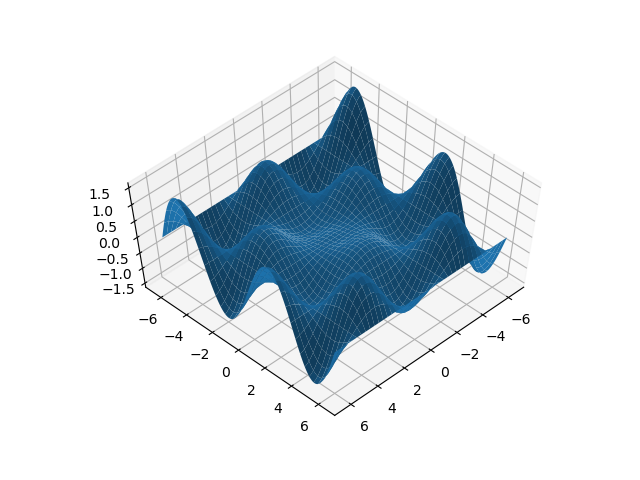
\includegraphics[width=.6\linewidth]{./gfx/np-wave}
	\captionof{figure}{Wellen auf Wasser}
\end{center}
\end{tcolorbox}

\section{Reduktion}
NumPy bietet viele Lösungen für Operationen auf Arrays. Wir kennen bereits Möglichkeiten, eine Berechnung für jedes Element eines Arrays auszuführen und dabei ein neues Array von Werten zu erhalten. Oft wollen wir aber die Werte nicht isoliert betrachten, sondern aus ihrer Gesamtheit einen einzigen Wert wie \eg. den Durchschnitt generieren. Auch für solche \emph{Reduktionen} bietet NumPy vorgefertigte Lösungen.

Natürlich kennen wir bereits Möglichkeiten, solche Reduktionen mit Python-Mitteln durchzuführen. Pythons \inPy{sum} und \inPy{len} geben Summe und Länge eines Arrays aus, und können auch auf NumPy-Arrays angewandt werden. Da diese Funktionen jedoch für sehr viele verschiedenartige Strukturen funktionieren sollen, konnten sie nicht weit optimiert werden. Aus diesem Grund bringt NumPy seine eigenen Funktionen mit, die die spezielle Struktur von NumPy-Arrays ausnutzen, und so eine Aufgabe sehr schnell lösen.

\begin{hintbox}[Exkursion: Zeitmessung mit \texttt{time}]
Das Modul \texttt{time} erlaubt -- wie es der Name schon suggeriert --, in Python mit Zeiten umzugehen. Neben Funktionen zur Formatierung von Zeitpunkten als Strings und Berechnung von Zeit-Abständen existiert die Funktion \texttt{time}, die das aktuelle Datum und Uhrzeit als Rückgabewert liefert. Diese Information wird in einer einzigen Fließkommazahl codiert, welche als Anzahl der Sekunden seit Mitternacht, erster Januar 1970 zu deuten ist. Vorteil dieser Konvention ist, dass solche \emph{Zeitstempel} einfach voneinander subtrahiert werden können, um \emph{Zeitabstände} zu erfahren.

Um den Zeitbedarf eines Algorithmus experimentell zu ermitteln hält man sich häufig an das folgende Schema:
\begin{codebox}[Schema: Zeitbedarf ermitteln]
\begin{minted}{python3}
import time

R = 1000

tic = time.time()
for run in range(R) :
    # Algorithmus
toc = time.time()

print(f"it took {toc - tic} second to run the algorithm {R} times")
\end{minted}
\end{codebox}

Die sehr kleinen Zeiten, die ein Computeralgorithmus zur Durchführung braucht, sind oft starken Schwankungen unterworfen. Um diese Schwankungen auszugleichen, wird meist nicht der Zeitbedarf für \emph{einen} Durchlauf ermittelt, sondern der Bedarf für \emph{sehr viele} Durchläufe des Algorithmus. Hieraus erklärt sich die \inPy{for}-Schleife im obigen Schema.
\end{hintbox}

Ein kurzes Script illustriert, wie viel größer der Zeitaufwand ohne Python-Funktionen ist:

\begin{codebox}[Beispiel: Zeitbedarf Array-Summation mit NumPy und Python]
\begin{minted}[linenos]{python3}
import numpy as np
import time

N = 10000
R =  2000
X = np.linspace(0, 100, N)
\end{minted}
\end{codebox}
%
\begin{codebox}[]
\begin{minted}[linenos, firstnumber=last]{python3}
print(f"taking the time for summation of {N} values, Python-Style...",
      end="", flush=True)
tic = time.time()
for run in range(R) :
  s = sum(X)
toc = time.time()
print("done")
tPython = toc - tic

print(f"taking the time for summation of {N} values, NumPy-Style...",
      end="", flush=True)
tic = time.time()
for run in range(R) :
  s = np.sum(X)
toc = time.time()
print("done")
tNumpy = toc - tic

print()
print(f"Measured {tPython*1000/R:5.3f} milliseconds using the Python-Method")
print(f"Measured {tNumpy *1000/R:5.3f} milliseconds using the NumPy-Method")
print(f"NumPy is {tPython/tNumpy:5.1f} times faster than native Python")
\end{minted}
\end{codebox}
%
\begin{cmdbox}[Ausgabe: Zeitbedarf Array-Summation mit NumPy und Python]
\begin{minted}{text}
taking the time for summation of 10000 values, Python-Style...done
taking the time for summation of 10000 values, NumPy-Style...done

Measured 1.589 milliseconds using the Python-Method
Measured 0.008 milliseconds using the NumPy-Method
NumPy is 211.5 times faster than native Python
\end{minted}
\end{cmdbox}

Bei mehrdimensionalen Arrays wird standardmäßig über alle Einträge summiert. Optional kann aber auch der \inPy{int}-Parameter \texttt{axis} mitgegeben werden. Dieser gibt an, über die wievielte Dimension summiert werden soll. Auch der Rückgabetyp des hierbei entstehenden NumPy-Arrays kann über das optionale Argument \texttt{dytpe} bestimmt werden.

\begin{tcbraster}[raster columns=2,
                  raster equal height,
                  nobeforeafter,
                  raster column skip=0.5cm]
\begin{codebox}[Beispiel: Zeitbedarf Array-Summation mit NumPy und Python]
\begin{minted}[linenos]{python3}
import numpy as np

npTab = np.array([[1, 2], [3, 4]])

print( np.sum(npTab) )
print( np.sum(npTab, axis=0) )
print( np.sum(npTab, axis=1) )
\end{minted}
\end{codebox}
%
\begin{cmdbox}[Ausgabe: Zeitbedarf Array-Summation mit NumPy und Python]
\begin{minted}{text}
10
[4 6]
[3 7]
\end{minted}
\end{cmdbox}
\end{tcbraster}

Das eben zu \texttt{np.sum} gesagte gilt so gleichermaßen auch für \texttt{np.prod} (Produkt der Werte eines NumPy-Arrays).

Der Mittelwert eines NumPy-Arrays kann über \texttt{mean} ermittelt werden. Auch hier können optional \texttt{axis} und \texttt{dtype} mit angegeben werden. Eine Erweiterung von \texttt{mean} stellt \texttt{average} dar. Diesem kann ein optionaler Parameter \texttt{weights} mitgegeben werden. Wie der Name nahelegt, handelt es sich hierbei um Gewichte für die einzelnen Werte des Daten-Arrays. Der Aufruf \texttt{np.average(a, weights=w)} berechnet also
\[ \frac{\sum_i a_i w_i}{\sum_i w_i}\]

Der Nenner in diesem Ausdruck -- die sogenannte \emph{Zustandssumme} oder \emph{Partition Function} -- kann mit demselben Befehl in Erfahrung gebracht werden. Wird das optionale Argument \inPy{returned=True} mit übergeben, so ist der Rückgabewert ein \inPy{tuple} aus gewichtetem Durchschnitt und Zustandssumme\footnote{Ich \emph{hasse} Thermodynamik.}:

\begin{codebox}[Beispiel: Durchschnittgeschwindigkeit in Wasserstoff (Statistische Physik)]
\begin{minted}[linenos]{python3}
import numpy as np

kB = 1.380649e-23         # Boltzmann constant
T  = 300                  # Temperature in Kelvin
m  = 2 * 1.6735575e-27    # hydrogen molecule mass in kg

velocities = np.linspace(0, 5000, 50000)
energies   = m/2 * velocities**2
w = np.exp(-energies / (kB * T))

vMean, Z = np.average(velocities, weights=w, returned=True)

print("weighted average:", vMean)
print("partition function:", Z)
\end{minted}
\end{codebox}
%
\begin{cmdbox}[Ausgabe: Durchschnittgeschwindigkeit in Wasserstoff (Statistische Physik)]
\begin{minted}{text}
weighted average: 887.5169329420108
partition function: 13942.18222351434
\end{minted}
\end{cmdbox}

mean und average
std
median
min, max


\section{Array-Operationen}
concatenate, stack, split, tile, repeat, delete, insert, resize, reshape, roll, sort, argmax, argmin
%https://numpy.org/doc/stable/reference/routines.array-manipulation.html

\section{Lineare Algebra}
dot, inner, outer, matmul (@), linalg.matrix\_power(a, n), linalg.solve
% https://numpy.org/doc/stable/reference/routines.linalg.html

\section{Polynome}
Poly1D Class
% https://numpy.org/doc/stable/reference/routines.polynomials.html

\section{Outlook}
%https://numpy.org/doc/stable/reference/index.html